\documentclass{article}
\usepackage{nips13submit_e,times}
\usepackage[utf8x]{inputenc}
\usepackage{amsfonts}
\usepackage{indentfirst}
\usepackage{hyperref}
\usepackage{graphicx}
\usepackage{enumerate}
\usepackage{amsmath}
\usepackage{subfigure} 
\usepackage{amsopn}
\title{Project-I by group TORONTO}
\author{Michalina Pacholska \And Jakub Sygnowski}
\nipsfinalcopy
\begin{document}
\maketitle
\begin{abstract}
This raport describes our work on first project done for Machine Learning class at EPFL in Fall 2014. We were given two synthetic datasets - a regression and a classification one and used methods learnt in the class to train few models and predicted regression and classification outcome for the test data we got. For classification, we tried fitting logistic regression, its penalized version and SVM. We achieved the best test error for penalized logistic regression with all input variables and their absolute values. For regression, we found out our data matrix is ill conditioned, the reason of which were discrete input variables. We removed them and then fit least squares with both gradient descent and normal equations and ridge regression. Ridge regression did not give us significant improvement over least squares and we used the latter model to predict the outcomes.
\end{abstract}

\begin{section}{Classification}
\begin{subsection}{Data preparation}
Our dataset consists of train data, for which we have both input variables $X$ and output $y$ and test data, for which we observe only $X$ and have to produce our predictions and approximation of certainity.

Both original train and test data sets included $N=1500$ samples, each has $33$ dimensions. All except $3$-rd input variable are continuous, $3$-rd is a binary one. Our $X_train$ matrix has full-rank, so we don't expect one input variable to be a linear function of other ones. 
Data we got was not normalized, as shown in figure \ref{fig:boxplotBefore}, so we decided to normalize it. We also normalized test data using same means and standard deviations. After that, we randomly a subset of $N=70$ data samples to leave it aside and use it at the end to estimate RSME error without being biased because of using cross-validation. 

Figure \ref{fig:boxplotBefore} shows also that our data is not free of outliers. We decided to remove from dataset all samples that have absolute value of any input variable $\ge 5$ standard deviations of this input variable (after normalization).

After these procedures, we end up with normalized data shown on figure \ref{fig:boxplotAfter}. There was $N=1284$ data samples left available to train our model.

\begin{figure}[!h]
\center
\subfigure[Boxplot of original input data $\mathbf{X}$. Data is not centered and therefore we normalize it.]{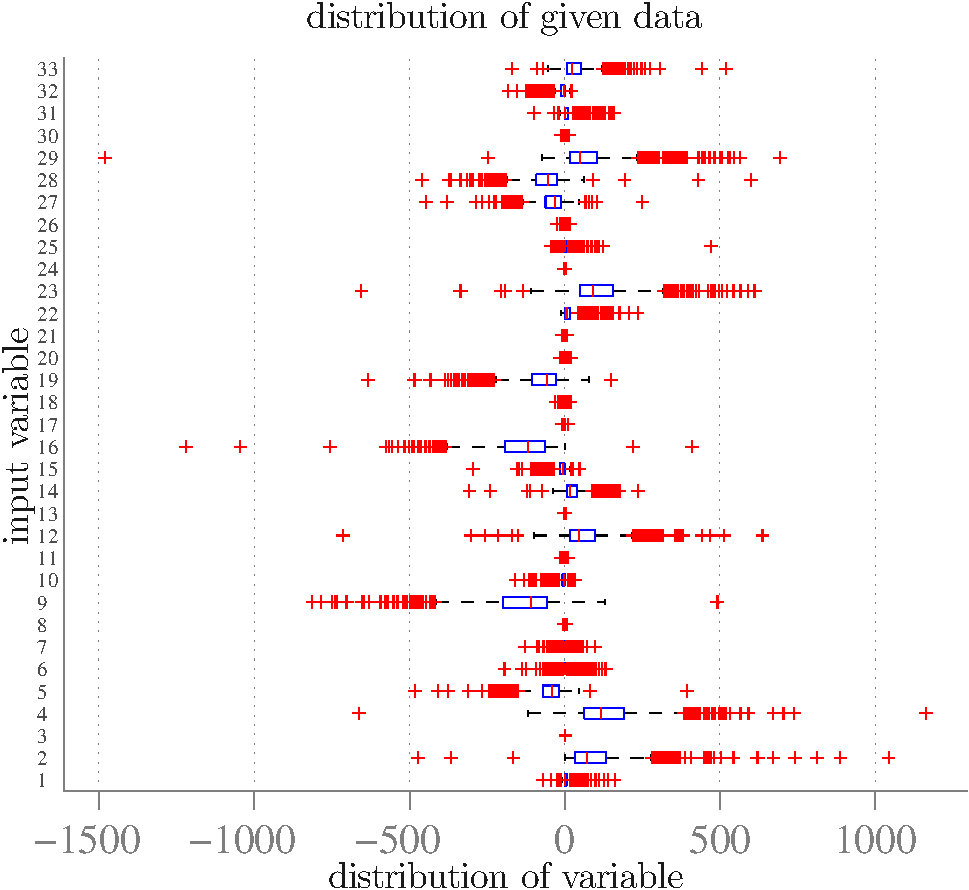
\includegraphics[width=2.5in]{../figures/classif/boxplot_before-crop.pdf} \label{fig:boxplotBefore}}
\hfill
\subfigure[Boxplot of input data after normalization and removing outliers.]{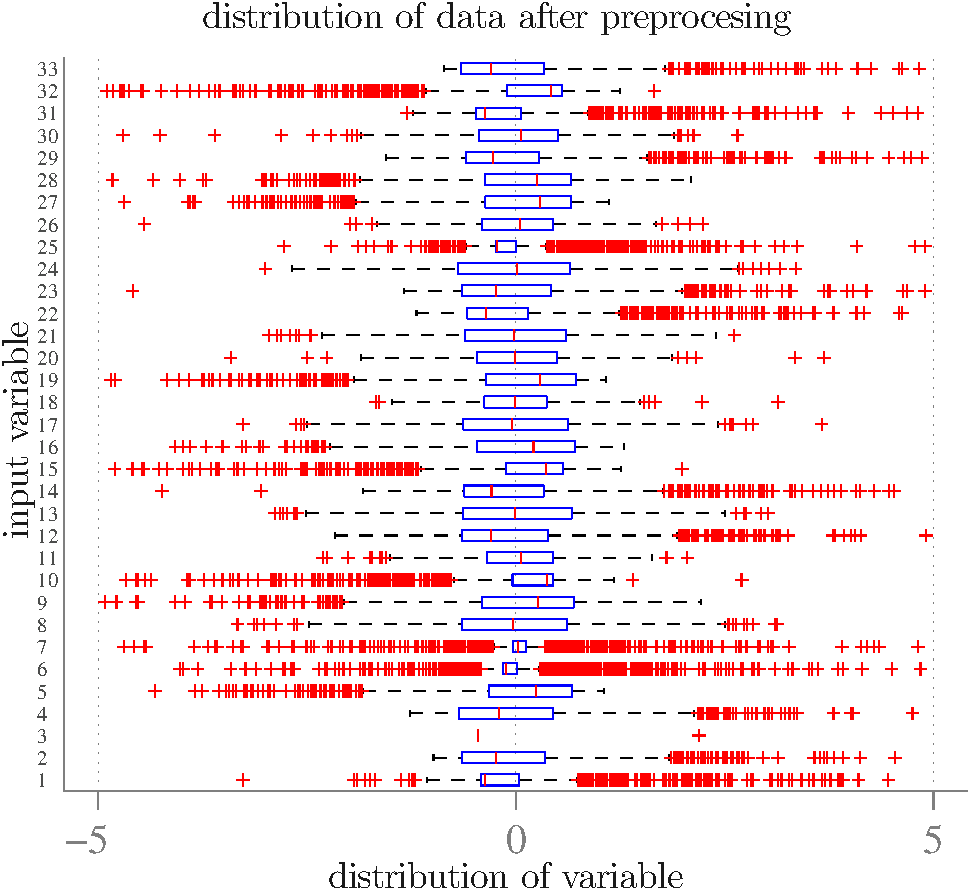
\includegraphics[width=2.5in]{../figures/classif/boxplot_after-crop.pdf} \label{fig:boxplotAfter}}
\caption{}
\end{figure}

\end{subsection}
\begin{subsection}{Data analysis}
We investigated correlation between different input variables and an output variable and amongst input variables themselves. Figure \ref{fig:correlation} shows that some variables are clearly more correlated to the output then the others. While building models we sometimes tried to create them only using few most correlated variables. On the other hand, we found no interesting correlation between input variables. We also tried to apply PCA to extract principal components of the data, but we found that particular principal components are not so well correlated with output variable (see fig. \ref{fig:pca}), so we abandoned this path and did not use PCA later.

\begin{figure}[!t]
\center
\subfigure[Correlation between input variables and output variable. Some variables have much bigger correlation to the output variable than the others.]{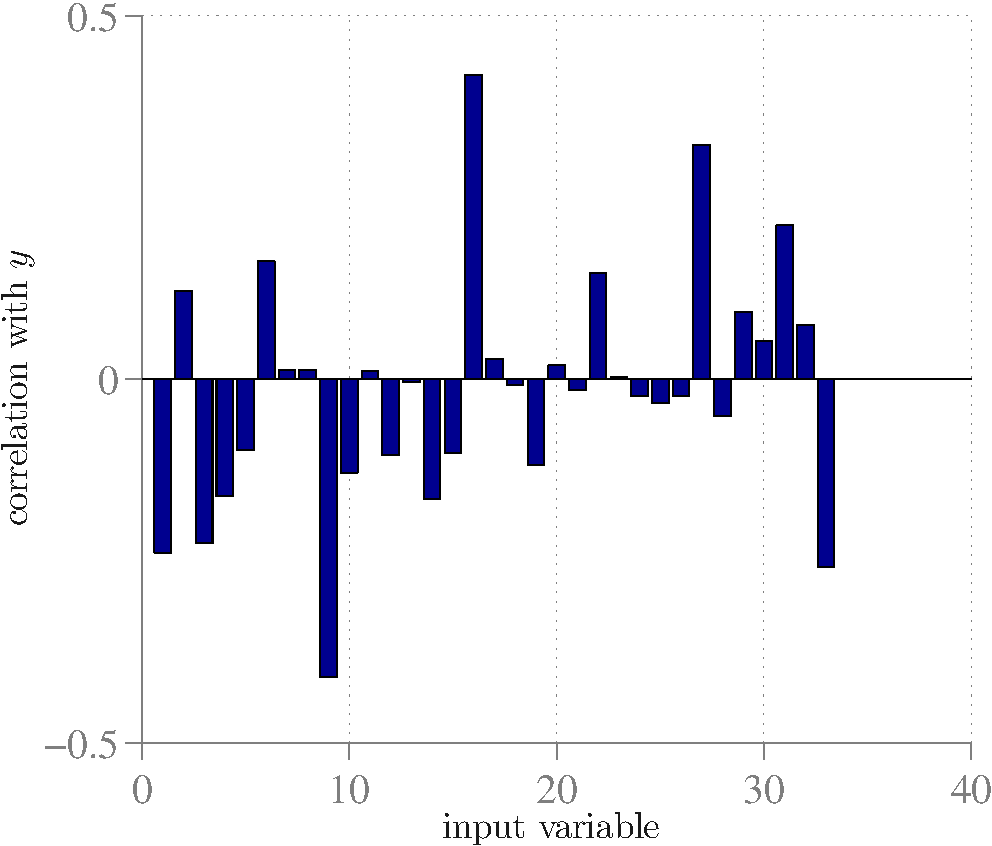
\includegraphics[width=2.5in]{../figures/classif/bar_ycorrelation-crop.pdf} \label{fig:correlation}}
\hfill
\subfigure[Data transformation using PCA. Big correlation of some input variables with $y$ is lost.]{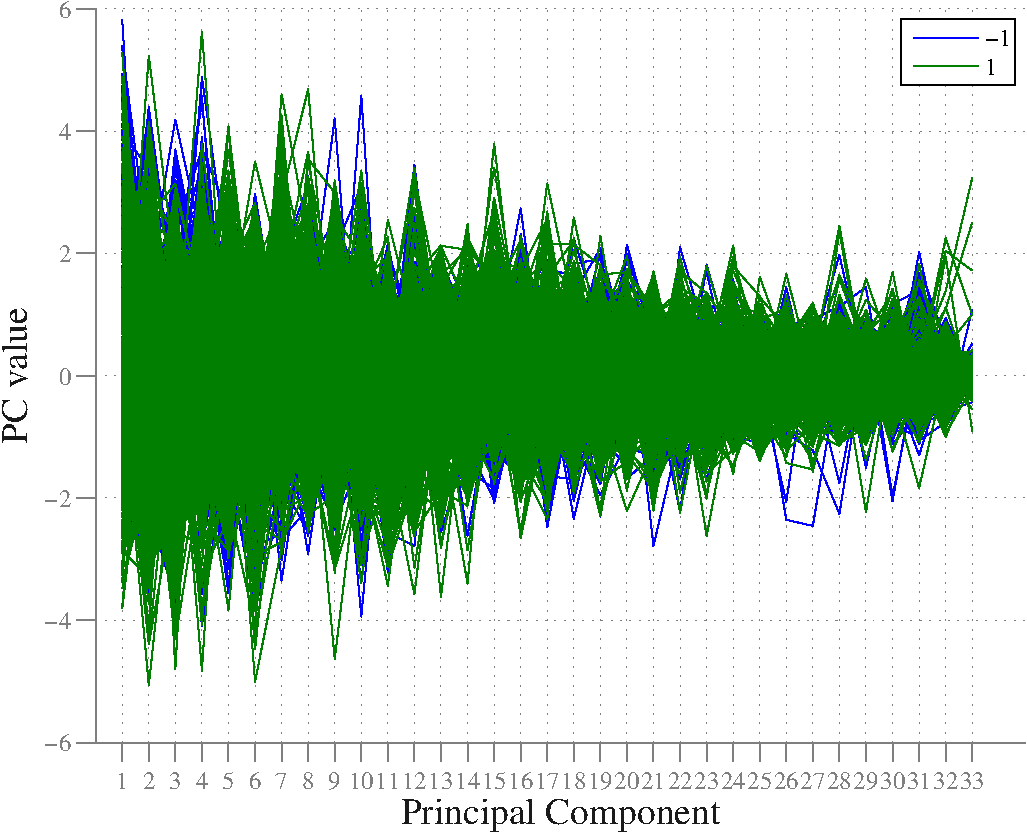
\includegraphics[width=2.5in]{../figures/classif/parallelcoords-pca-crop.pdf} \label{fig:pca}}
\caption{}
\end{figure}

\end{subsection}
\begin{subsection}{Predicting models}
\begin{subsubsection}{Logistic regression using gradient descent}
First model we tried to fit was simple logistic regression (using Newton's method with Hessian). Using $10$-fold cross-validation, we achieved mean logistic test error of $0.2301$. The results had big variance. We later tried to fit the model using only $9$-th input variable (the one with biggest correlation with output), but it got worse test error.

\end{subsubsection}
\begin{subsubsection}{Penalized logistic regression}
We did a lot of experiments using penalized logistic regression. As converging using gradient descent was slow, we wrote a Hessian-based version.

To choose optimal value of $\lambda$, we used $10$-fold cross-validation. We tested $200$ candidates in logspace between $10^{-2}$ to $10^2$. Figure \ref{fig:lambda} shows the result: optimal lambda was $\lambda = 0.8$ with test error around $0.19$.

\begin{figure}[!t]
\center

\subfigure[Train and test error of penalized logistic regression without transformations for different value of $\lambda$]{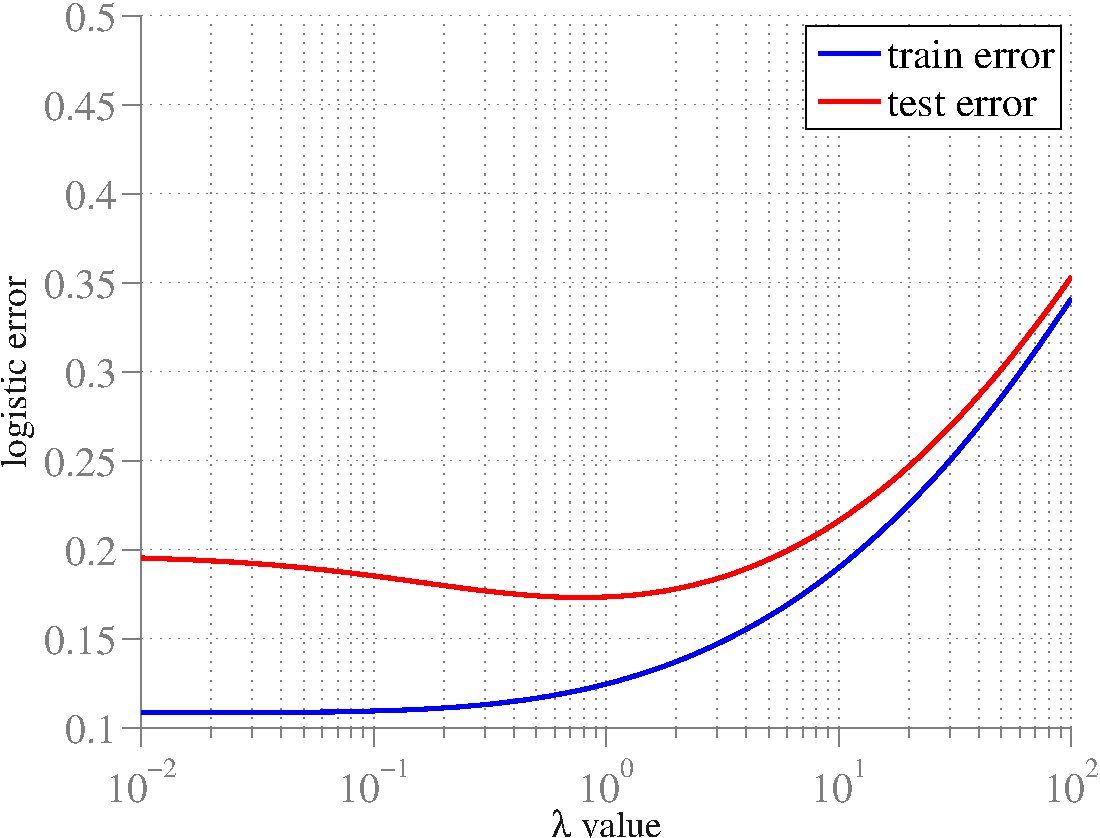
\includegraphics[width=2.5in]{../figures/classif/lambda-crop.pdf} \label{fig:lambda}}
\hfill
\subfigure[Comparison of train and test error for different value of $\lambda$ in model with absolute value of input variables]{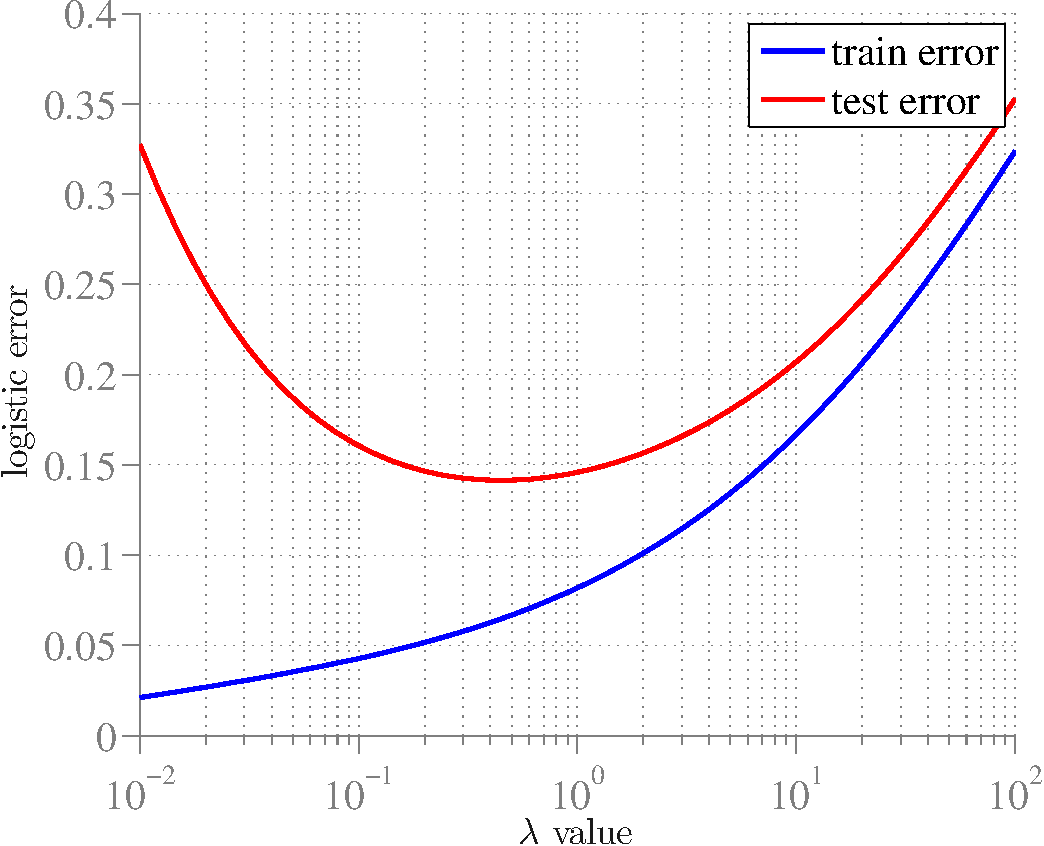
\includegraphics[width=2.5in]{../figures/classif/lambda_abs-crop.pdf} \label{fig:lambda-abs}}
\caption{}
\end{figure}

\begin{subsubsection}{Feature transformations}
Later, we tried various feature transformations. We mention the ones which did not get any improvement in no significant order:
\begin{itemize}

\item running penalized logistic regression for only some ($\{1, 9, 16, 27, 33\}$) of input variables with biggest correlation to the output variable
\item penalized log. regression for subset of variables and their squares and square roots
\item penalized log. regression with all input variables and their square roots
\item penalized log. regression with all input variables and their cubes
\end{itemize}

On the other hand, we got similiar improvement (logistic error went down to around $0.15$) for both adding squares and absolute value of every input variable. The result of cross-validation for different $\lambda$ and all variables and their absolute value is shown on figure \ref{fig:lambda-abs}. As expected, we observe increase in test error for small value of $\lambda$ (variance), but overall, for $\lambda = 0.5$.
\end{subsubsection}
\end{subsubsection}
\begin{subsubsection}{SVM}
We also tried to fit (builtin) SVM model for our problem. Unfortunately, when we chose only a subset of input variables we got bigger error then before, and when we tried to fit SVMs for all input data, training never finished. Changing the kernel didn't help.
\end{subsubsection}
\end{subsection}
\begin{subsection}{Summary}
After fitting the mentioned models, we found out that most of input variables have an inpact on predicting the outcome $y$. Our logistic regression test error ($0.18$) was on average bigger than the penalized regression one ($0.15$), so we decided to use penalized logistic regression to predict the unknown outcomes. We did not managed to make SVM work for all the features due to its computational complexity.
\end{subsection}
\end{section}
\begin{section}{Regresssion}
\begin{subsection}{Data preparation}
For the regression problem, we got input data matrix $X$ with $N=1400$ data samples and $D = 52$ input variables. First $38$ of input variables are continuous, last $14$ are discrete, with more than $2$ categories. $X$ matrix is again full-rank. Figure \ref{fig:boxplot_reg_before} shows that data is again not normalized, especially $38$-th column. 

\begin{figure}[!h]
\center
\subfigure[Boxplot of original input data $\mathbf{X}$. Data is not normalized and categorical variables are not separated]{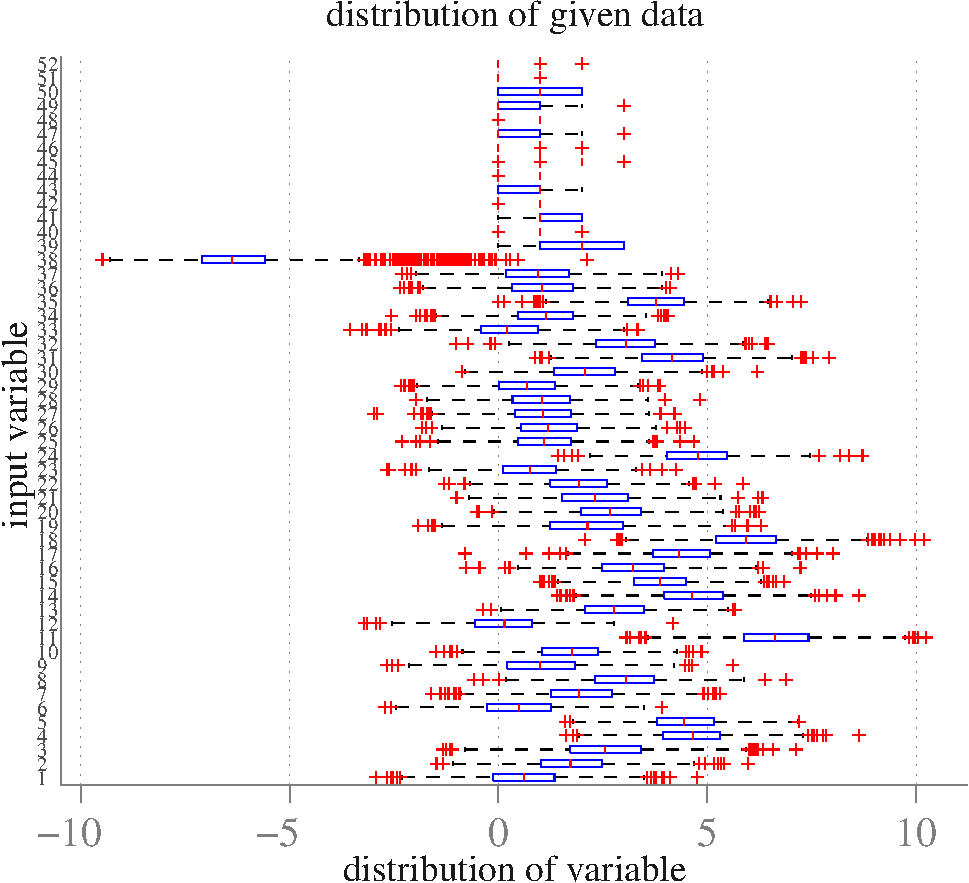
\includegraphics[width=2.5in]{../figures/boxplot_before_r-crop.pdf} \label{fig:boxplot_reg_before}}
\hfill
\subfigure[Correlation of input variables with the output variable]{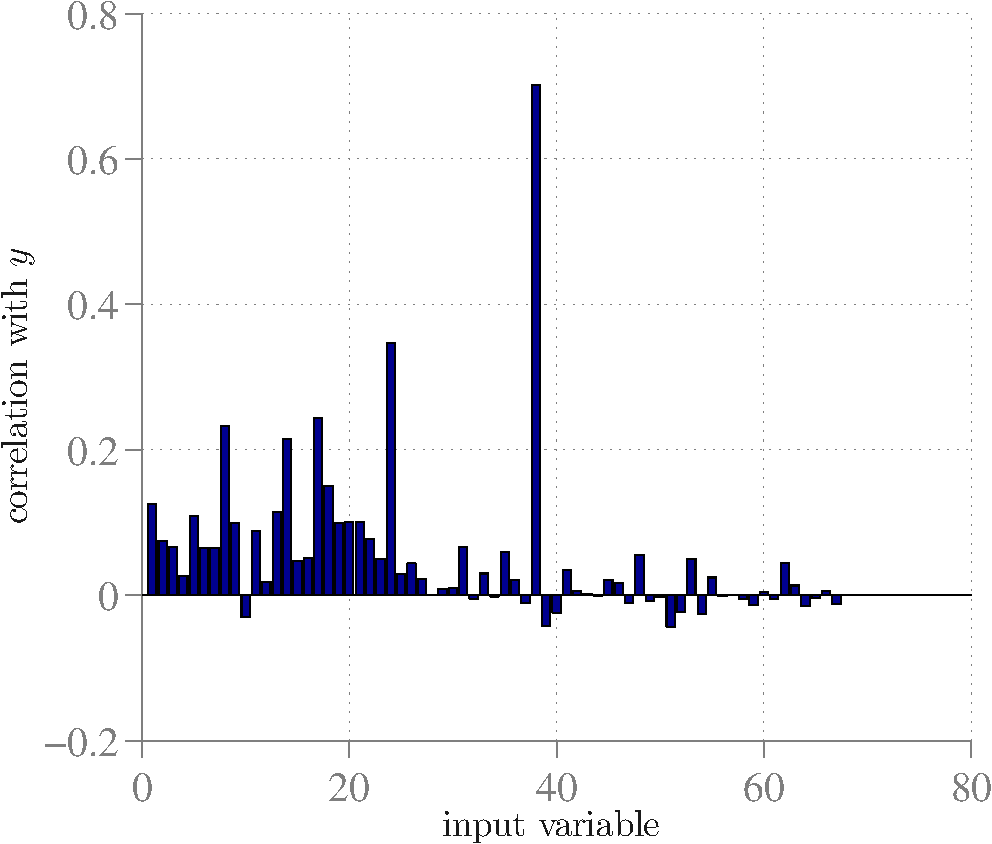
\includegraphics[width=2.5in]{../figures/correlation-crop.pdf} \label{fig:correlationReg}}
\caption{}
\end{figure}
\begin{subsubsection}{Dummy encoding}
First procedure which we applied to our data is dummy encoding of categorical variables. After changing variables to binary, we had matrix $X$ with $80$ columns but only $67$ rank, which means that there was some redundancy in categorical variables. To avoid problems with ill-conditioning, we chose $67$ linearly independent columns of $X$ and discarded others.
\end{subsubsection}

Further, we normalized the data and removed sample case \#$500$ as an outlier.
\end{subsection}
\begin{subsection}{Data analysis}
We took a look at the correlation between input variables, and there was not much correlation. More interesting was correlation of each input variable with the output one, which is shown on the figure \ref{fig:correlationReg}. We clearly see that there's a big correlation between $38$-th input variable and our output, but if we took a look at the plot of this variable vs $y$ (fig. \ref{fig:38-cor}) we see that data is in fact clustered and big correlation may not guide us to very good predictions.
\begin{figure}[!h]
\center
\subfigure[Plot of $38$-th input variable vs output variable. We see the clusterization of the data separated. Fit is good for one cluster, but not for the second one.]{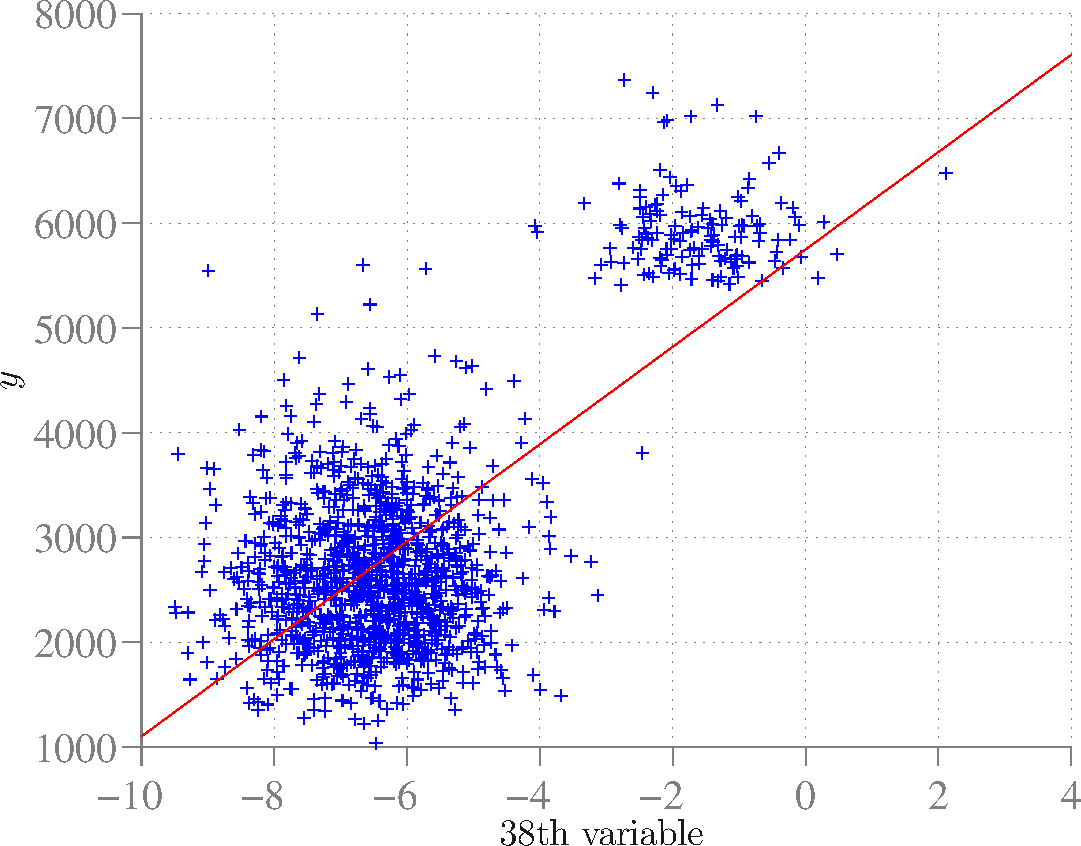
\includegraphics[width=2.5in]{../figures/variable38-crop.pdf} \label{fig:38-cor}}
\hfill
\subfigure[Train and test error for different values of $\lambda$ in ridge regression. We see that penalizing big $\beta$ values is not justified.]{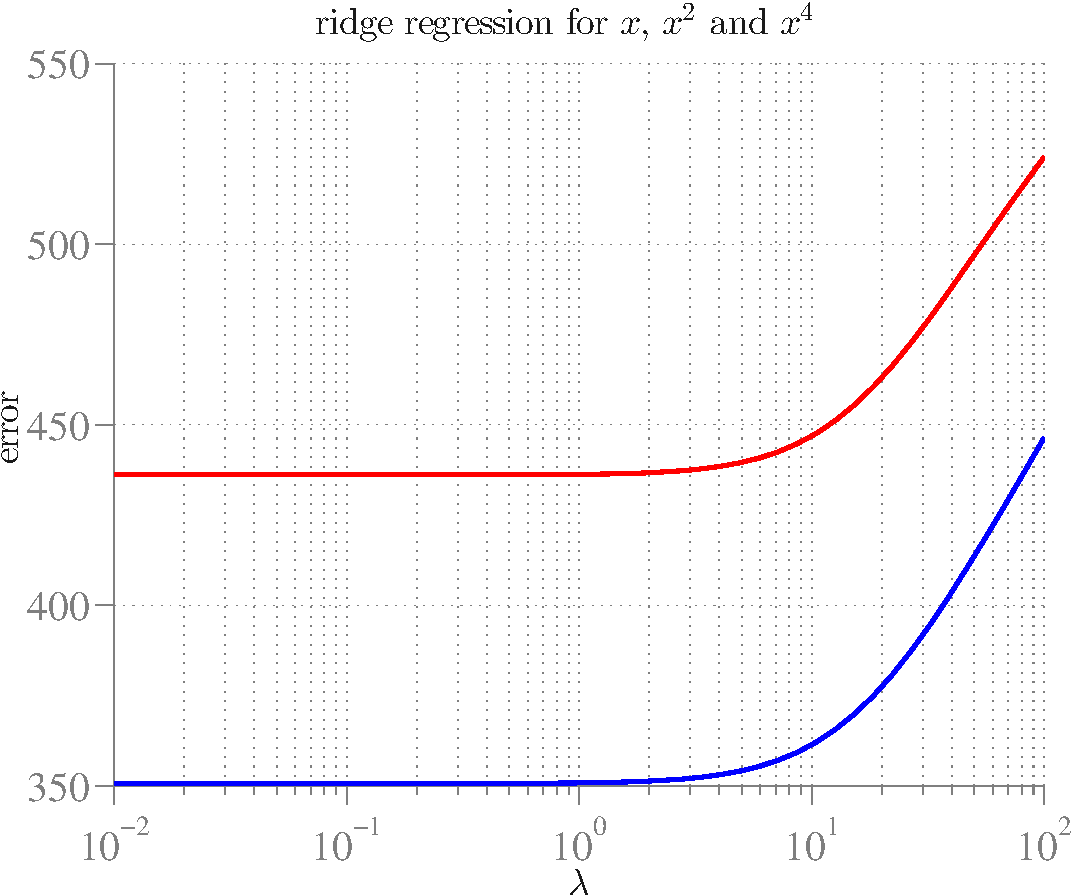
\includegraphics[width=2.5in]{../figures/ridge-crop.pdf} \label{fig:ridge}}
\caption{}
\end{figure}
\end{subsection}
\begin{subsection}{Least squares and feature transformations}
We started by analysing the behaviour of least squares under $10$-fold cross-validation. We run each testing case for $10$ choices of seeds and averaged the results. Testing cases were:
\begin{itemize}
\item all input variables, like we got them: $rsme=641$
\item all input variables and squares of continuous ones ($\{1, \ldots, 38\}$), $rsme = 59$
\item only continuous variables and their squares: $rsme = 471$
\item only continuous variables, their squares and fourth powers: $rsme = 469$
\end{itemize}
This was not very suprising, as:
\begin{enumerate}
\item we had badly conditioned matrix $X$, only because of our discrete variables, which could lead to computational errors when solving normal equations with all variables,
\item discrete variables were very lightly correlated with output variable, so removing them did not made us lost much of information.
\end{enumerate}
\end{subsection}
\begin{subsection}{Gradient descent}
Running gradient descent for this dataset was problematic. We for step size $\alpha > 0.2$ it did not converge, and at the same time it was taking a lot of time to converge using smaller step sizes. Removing discrete variables again helped, and we managed to make it converge using continuous variables and their squares by making even smaller step size, but results were very similar to those achieved by using normal equations, so we decided to not use gradient descent later.

\end{subsection}
\begin{subsection}{Rigde regression}
We tried to fit ridge regression for different values of $\lambda$ and tried various feature transformations. It turned out (fig. \ref{fig:ridge}) that model works best when $\lambda$ is set to zero and features are chosen the same way as with least squares method. Amongst others, we also tried fitting ridge regression to all continuous variables and their pairwise multiplication pairs, but we made our model overfitting, as shown in the figure \ref{fig:ridgeAllPairs}.
\begin{figure}[!h]
\center
\subfigure[Errors for ridge regression model with all second order terms. Big difference of train and test error tells us that our model has big variance.]{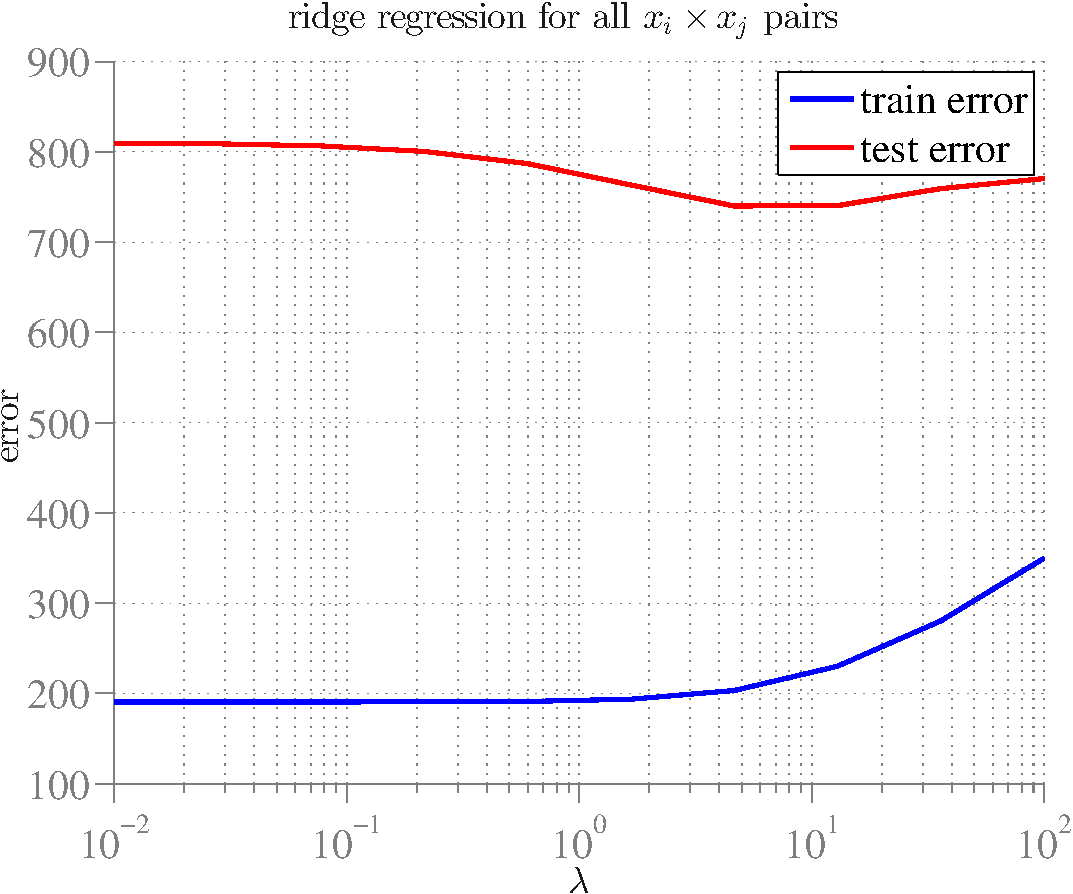
\includegraphics[width=2.5in]{../figures/ridgeAllPairs-crop.pdf} \label{fig:ridgeAllPairs}}
\hfill
%\subfigure[Train and test error for different values of $\lambda$ in ridge regression. We see that penalizing big $\beta$ values is not justified.]{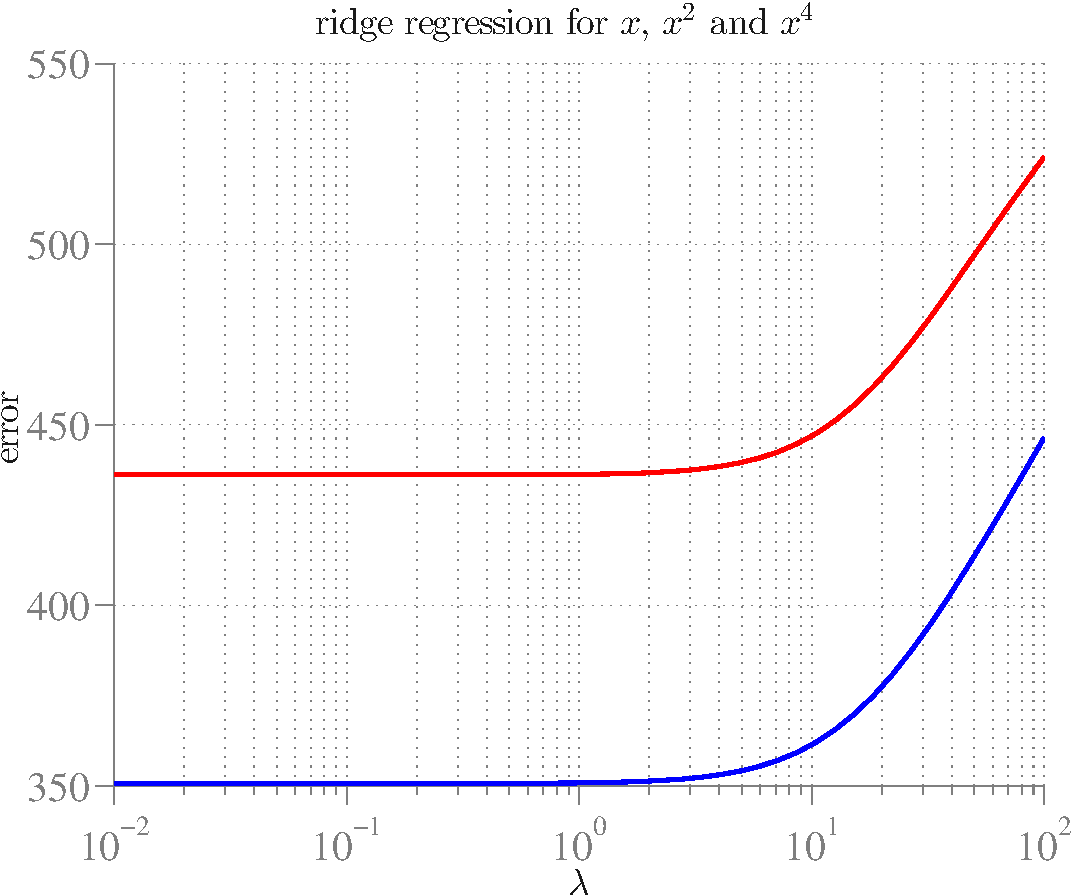
\includegraphics[width=2.5in]{../figures/ridge-crop.pdf} \label{fig:ridge}}
\caption{}
\end{figure}
\end{subsection}
\begin{subsection}{Summary}
We found out that using of discrete input variables in predicting the regression outcome increases the error and makes the matrix ill-conditioned. We dropped this variables completely and fit the least squares using normal equations and gradient descent and ridge regression for different values of $\lambda$. It turned out that all predictors (on model with input variables, their squares and $4$-th powers) give the same rsme test error of $442$, with the remark that convering gradient descent was hard due to setting the step size. Even in ridge regression, adding more variables guided us to overfitting. We finally used the normal equations predictor as the lightest computationally one.
\end{subsection}
\end{section}

\end{document}
